\documentclass[a4paper]{article}

\usepackage{graphicx}
\usepackage{parskip}
\usepackage{hyperref}

\author{A. Abdulwahed, M. Kaoula, M. Laruina, R. Mancini}
\title{Distributed Key Value Store using RAFT\\Final Documentation}
\date{\today}

\begin{document}

\pagenumbering{gobble}
\maketitle
\vfill
% \setcounter{tocdepth}{1}
\tableofcontents
\vfill
\clearpage
\setcounter{page}{1}
\pagenumbering{arabic}

\section{Introduction}

The goal of the project is to implement a distributed and strongly 
consistent in-memory key-value store using the RAFT algorithm for consensus 
among the different nodes.
The developed architecture (figure~\ref{fig:raft-arch}) is highly modular, leading to better flexibility and 
re-usability. With this choice, synchronization and coordination issues are 
offloaded to the communication between the modules.

\begin{figure}[b]
    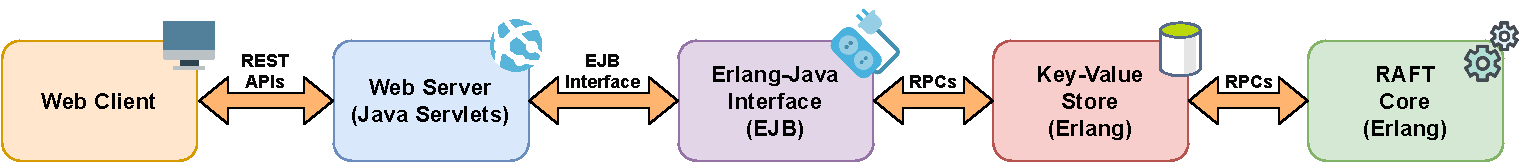
\includegraphics[width=\textwidth]{raft_architecture.pdf}
    \caption{High-level architecture of the project.}
    \label{fig:raft-arch}
\end{figure}

The possible operations on the distributed KV store will be the following:
\begin{itemize}
    \item \texttt{V get(K key)}: returns the value associated with the key
    \item \texttt{Map<K,V> getAll()}: returns all key-value pairs
    \item \texttt{void set(K key, V value)}: sets the given value to the 
        provided key
    \item \texttt{void delete(K key)}: deletes the item with the given key
    \item \texttt{void deleteAll()}: deletes all the keys
\end{itemize}

The core of the RAFT algorithm will be developed using Erlang and will be 
generic (section \ref{sec:raft-core}). Using this generic RAFT implementation, 
another Erlang RPC server will be developed which implements the Key-Value 
store (section \ref{sec:kv-store}) and provides an interface to access the 
datastore. Another module will make it possible to access the key-value 
store from Java, using the \emph{Jinterface} package 
(section \ref{sec:erlang-java}). 
This exported interface will be used by a web-server which will provide 
REST APIs for the key-value store and an administration GUI
(section \ref{sec:web-server}).

For comparison purposes, we will also develop a web server using Erlang Cowboy
framework, which will replace the Web Server and the Erlang-Java interface in 
figure~\ref{fig:raft-arch}.

\subsection{RAFT} 
Raft implements consensus by first electing a server as leader, then giving the leader complete
responsibility for managing the replicated log. The leader accepts log entries from clients, replicates
them on other servers, and tells servers when it is safe to apply log entries to their state machines.
Having a leader simplifies the management of the replicated log. For example, the leader can decide
where to place new entries in the log without consulting other servers, and data flows in a simple
fashion from the leader to other servers. A leader can fail or become disconnected from the other
servers, in which case a new leader is elected.

%=== DESIGN ===

\section{Design and Architecture}
In this section the overall architecture of the system is explained, as well
as the design of the principal modules.

\subsection{System Architecture}
\begin{figure}
    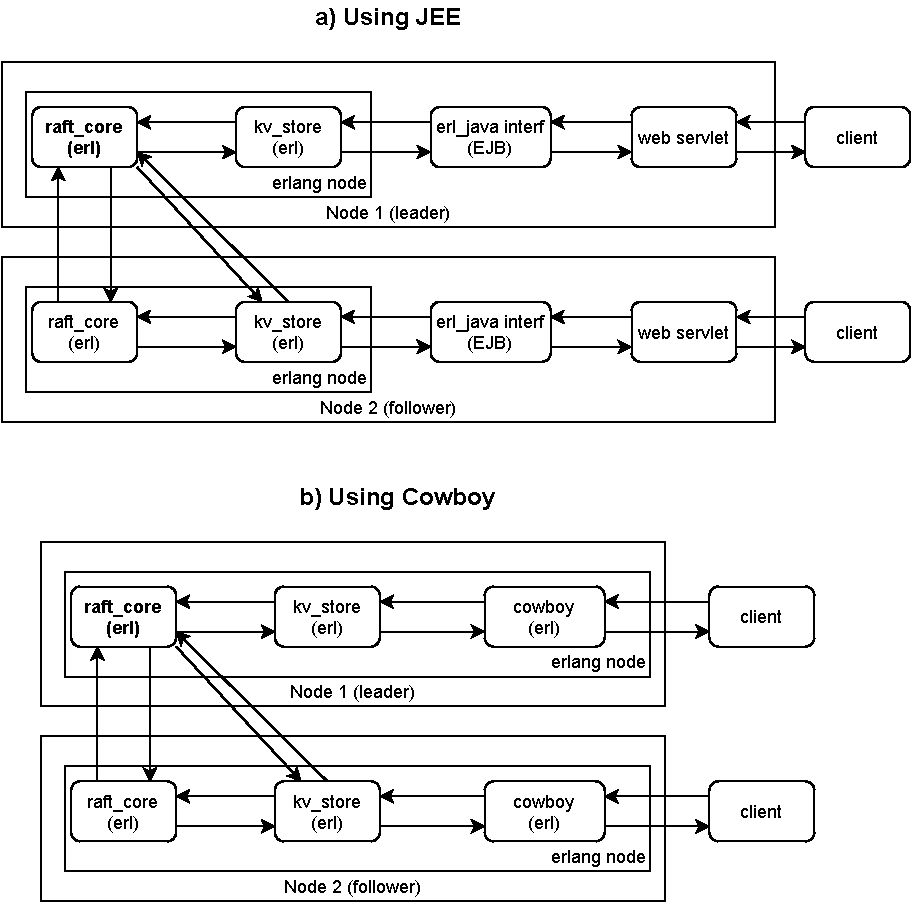
\includegraphics[width=\textwidth]{raft_arch2.pdf}
    \caption{Simplified representation of a possible deployment with either Glassfish (using JEE) or Cowboy web server (in Erlang). Only two nodes are shown since all follower nodes are the same but at least 3 nodes are required (an odd number of nodes is recommended).}
    \label{fig:raft-arch2}
\end{figure}

In figure~\ref{fig:raft-arch2} the target architecture of the system is shown, 
in particular:
\begin{itemize}
    \item different RAFT instances run on different (physical) nodes.
    \item on each Erlang node, both the RAFT and KV-Store processes are hosted.
        These two modules will communicate using local RPCs.
    \item in case of JEE, the jinterface module will run on a separate Erlang 
        node located on the same physical node. On the same node, also an 
        instance of the web interface servlet will run (e.g. using Glassfish).
    \item in case of Cowboy, also the cowboy process will run on the same 
        Erlang node as the other two processes.
    \item clients will be able to connect to any of the servers, e.g. using 
        a load-balancer.
\end{itemize}

Due to this design, this distributed KV-Store implementation is suited to 
read-heavy applications that have a strong consistency requirements 
(e.g. configuration management systems).

\subsection{RAFT core}
\label{sec:raft-core}

\begin{figure}
    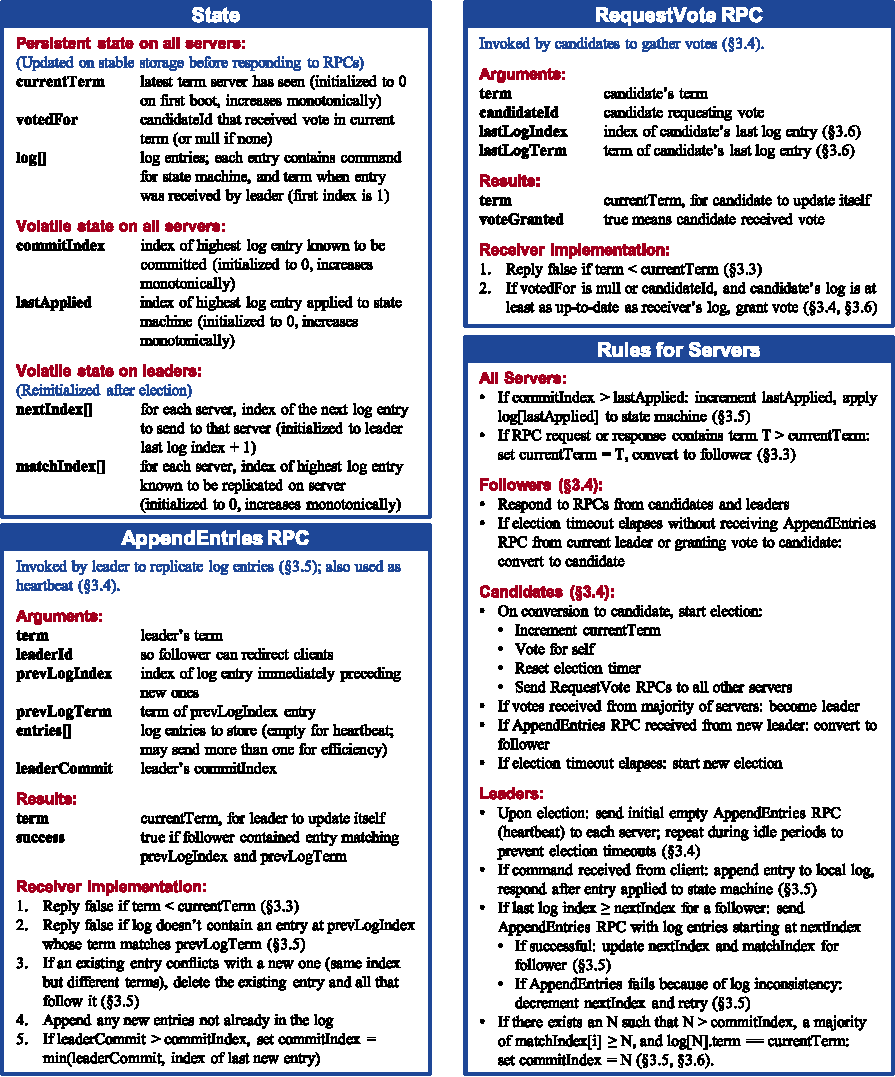
\includegraphics[width=\textwidth]{raft_algorithm.pdf}
    \caption{A condensed summary of the Raft consensus algorithm (excluding membership changes, log compaction, and client interaction). The server behavior in the lower-right box is described as a set of rules that trigger independently and repeatedly. (From original author's dissertation.)}
    \label{fig:raft-algorithm}
\end{figure}

This Erlang module will: 
\begin{itemize}
    \item implement the RAFT finite-state machine (FSM).
    \item take care of the replication of data between nodes.
    \item apply commits to the KV-Store module.
    \item persist its log on disk to reload its previous state on a crash.
\end{itemize}

The basic RAFT algorithm is shown in figure~\ref{fig:raft-algorithm}. Due to 
time constraints, more advanced features, such as membership changes and 
log compaction have not been implemented. For the same reasons, the 
implementation is not optimized for speed and efficiency. For more information
about the implementation of the RAFT module, refer to the ``Implementation''
section.

\subsection{KV store}
\label{sec:kv-store}

This Erlang module will implement the Key-Value store. It will need to 
handle incoming commits from the RAFT core and reply to get and set 
requests, querying the current master node\footnote{\emph{get} requests can 
be handled directly by a secondary node if a strong consistency is not 
required}. All communication with the Erlang core and the \emph{Erlang-Java
interface} will be done using RPCs.

\subsection{Erlang-Java interface}
\label{sec:erlang-java}

This Java module will expose the Erlang KV store to a JEE environment and 
will be implemented as an EJB. This EJB will provide an interface to 
view and edit the key-value store and will communicate with the Erlang 
environment through RPCs using the \emph{Jinterface} package. Communication
with other EJB will be handled by the JEE runtime.

\subsection{Web Server}
\label{sec:web-server}
This module is designed according to the Model-View-Controller (MVC) pattern, in particular:
there are three servlets working as controllers, they will have to receive HTTP requests from the web browser (client) and load the corresponding view requested by the http request.
Models will be responsible for interacting with the KV-Store through the interface offered by the EJB module.
The views contain the interfaces relating to the homepage and the page from which the KV-Store could be managed.

Also this module offers the same methods as the KV-Store but with interaction using JSON objects. This has been implemented to have the possibility of comparing the access performance to the system in the case in which a CowBoy server in Erlang and a REST API in Java is used.

\subsection{Erlang Web Server}
\label{sec:cowboy}
This module, as the previously described one, is designed according to the Model-View-Controller (MVC) pattern. It can be seen as an Erlang implementation of the Web Server (see \ref{sec:web-server}).
It will receive the user requests and reply accordingly. The replies will be
generated by querying directly the KV Store.
It listens to all the connection on a given port and provides an endpoint accepting \emph{GET}, \emph{POST}, \emph{PUT} and \emph{DELETE} requests from the users.

\subsection{Interactions}

\begin{figure}
    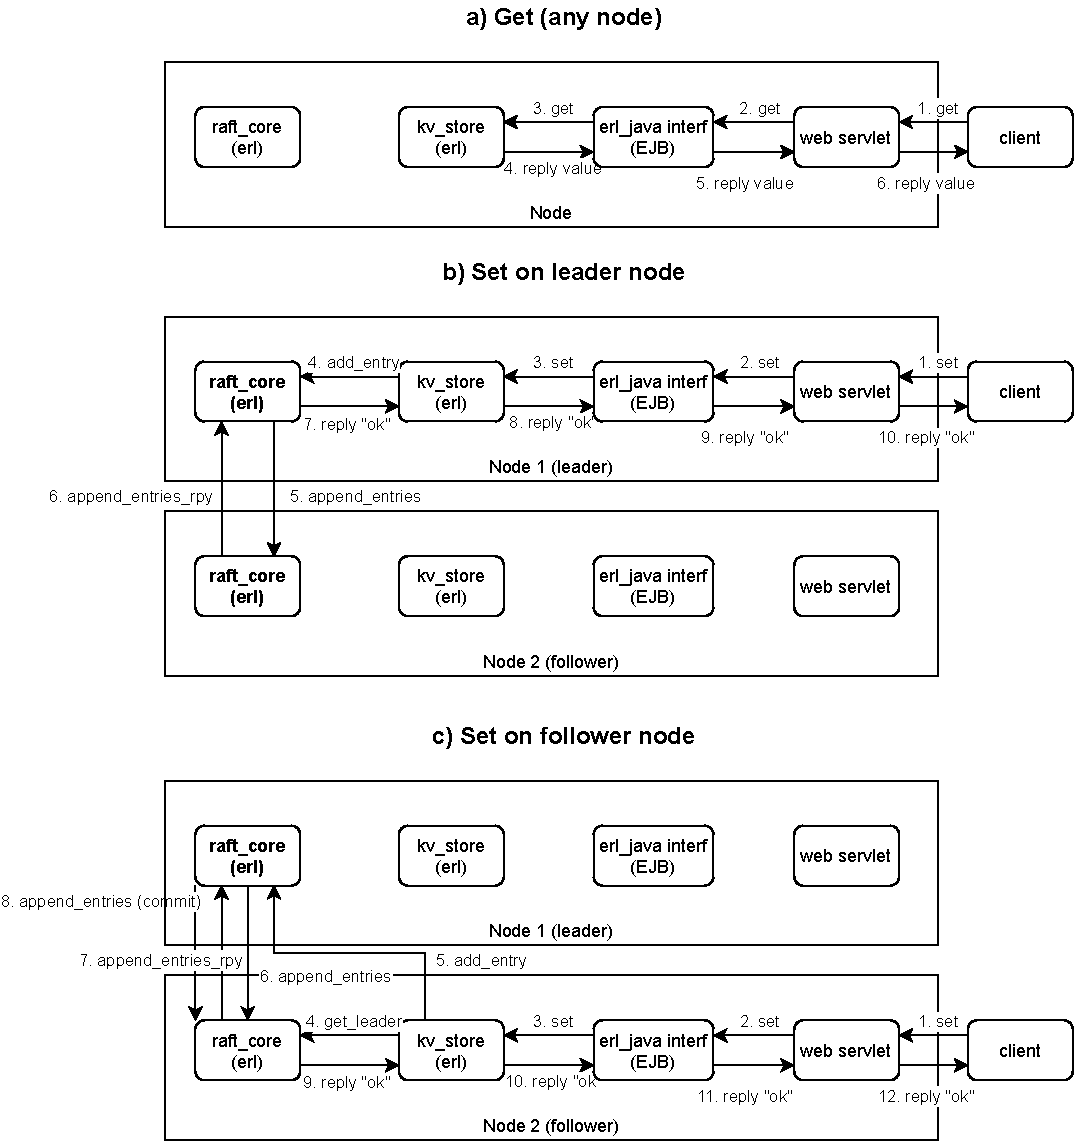
\includegraphics[width=\textwidth]{raft_operations.pdf}
    \caption{Activity diagram showing interactions between the modules in 
    case of a get or a set operation and in case of leader on same node of 
    web server or not.}
    \label{fig:raft-operations}
\end{figure}

In figure~\ref{fig:raft-operations}, you can see the interactions of the modules
in the case of a \emph{get} or an edit (in this case \emph{set}) request.

In particular, we can note that:
\begin{itemize}
    \item \emph{get} requests are handled by the local kv\_store, no matter if 
        it is the leader or not. This node may not be up-to-date with the 
        leader node but, eventually, it will be consistent with it. In 
        particular, a client talking with one node only will have a 
        consistent view on the data store (sequential consistency). However,
        there are no mechanisms put in place to guarantee the same consistency
        level if a client connects to multiple nodes\footnote{a naive solution 
        would be to force all requests to go through the leader; a better 
        solution would be to carry logical timestamps (aka the log index) 
        with the replies to the client.}
    \item \emph{set} requests always wait for the entry to be committed on the 
        local kv store. Remember that the leader will commit an entry only
        when it has successfully replicated it on a majority of nodes.
\end{itemize}

%=== IMPLEMENTATION ===

\section{Implementation}

\subsection{RAFT core}
The RAFT core Erlang module has been implemented the \emph{gen\_statem} OTP
behavior. In the following the most important implementation choices and 
differences from the theoretical algorithm are highlighted.

\paragraph{RPC implementation}
The RPCs defined in the RAFT algorithm have been implemented using 
a pair of \emph{casts} instead of a \emph{call}. This is due to the fact that
seeing it as a pair of events was more coherent with the state machine 
abstraction and thus was easier to implement. A missing reply or an incorrectly
ordered one does not impact on the correctness of the algorithm:
\begin{itemize}
    \item a late reply to \texttt{request\_vote} can be simply ignored.
    \item a missing reply to \texttt{request\_vote} means that the node is 
        crashed and therefore can be safely assumed as a negative answer.
    \item a late reply to \texttt{append\_entries} needs to be taken care of
        but in a very simple way (client needs to indicate its 
        \texttt{matchIndex} in the reply and the server should take the maximum
        between its local value and the received one since it is monotonically
        increasing).
    \item a missing reply to \texttt{append\_entries} means that the node is 
        crashed and therefore the node \texttt{matchIndex} will not be updated.
\end{itemize}

\paragraph{Messages for request\_vote ``RPC''}
\begin{itemize}
    \item \texttt{request\_vote\_req}
    \begin{itemize}
        \item \texttt{term}: candidate's term
        \item \texttt{candidate\_id}: candidate requesting vote
        \item \texttt{last\_log\_index}: index of candidate's last log entry
        \item \texttt{last\_log\_term}: term of candidate's last log entry
    \end{itemize}
    \item \texttt{request\_vote\_rpy}
    \begin{itemize}
        \item \texttt{term}: current term, for candidate to update itself
        \item \texttt{vote\_granted}: true means candidate received vote
    \end{itemize}
\end{itemize}

\paragraph{Messages for append\_entries ``RPC''}
\begin{itemize}
    \item \texttt{append\_entries\_req}
    \begin{itemize}
        \item \texttt{term}: leader's term
        \item \texttt{leader\_id}: so follower can redirect clients
        \item \texttt{prev\_log\_index}: index of log entry immediately preceding new ones
        \item \texttt{prev\_log\_term}: term of \texttt{prev\_log\_index} entry
        \item \texttt{entries}: list of log entrues to store (empty for heartbeat; may send more than one for efficiency)
        \item \texttt{leader\_commit}: leader's \texttt{commit\_index}
    \end{itemize}
    \item \texttt{append\_entries\_rpy}
    \begin{itemize}
        \item \texttt{term}: current term, for leader to update itself
        \item \texttt{success}: true if follower contained entry matching \texttt{prev\_log\_index} and \texttt{prev\_log\_term}
        \item \texttt{match\_index}: \texttt{prev\_log\_index}, so leaders can match replies with requests
    \end{itemize}
\end{itemize}

\paragraph{add\_entry RPC}
Issued by clients to add an entry to the replicated log.
\begin{itemize}
    \item parameters
    \begin{itemize}
        \item \texttt{entry}: the content of the entry to be added.
    \end{itemize}
    \item results
    \begin{itemize}
        \item \texttt{result}: ok or error. It can fail if node is not leader.
        \item \texttt{index}: index assigned to the entry (not yet committed).
        \item \texttt{term}: term of the entry.
    \end{itemize}
\end{itemize}

\paragraph{commit\_entry RPC}
Issued by the RAFT core to the client to ask for an entry to be applied.
\begin{itemize}
    \item parameters
    \begin{itemize}
        \item \texttt{index}: the index of the entry to be applied, so that the client can check if it is missing some.
        \item \texttt{term}: the term of the entry to be applied, so that the client can match with its previous \texttt{add\_entry} and reply to its clients.
        \item \texttt{entry}: the content of the entry to be applied.
    \end{itemize}
    \item results
    \begin{itemize}
        \item \texttt{result}: ok or error. It can fail if client is missing some entries.
        \item \texttt{index}: index of expected entry, if commit failed due to 
            mismatch. This is used by RAFT core to retry.
    \end{itemize}
\end{itemize}

\paragraph{Voting protocol}
When a node starts or becomes follower, the \emph{electionTimeout} timer is 
started (using a \texttt{state\_timer} in \texttt{gen\_statem}) with a 
random value in a configurable interval (in milliseconds). 
The timer will be reset every time an \texttt{append\_entries} from the 
rightful leader is accepted.
When the \emph{electionTimer} times out, the follower will become a candidate.
When doing so, it increases its term and it sends \texttt{request\_vote}
to all other nodes. The votes that have not cast a vote in this (new) term will
compare the last log entry information with 
the received one and will positively reply (using a \texttt{request\_vote\_rpy} 
cast) if the candidate's log is at least 
up-to-date as theirs. All other nodes will reply negatively. 
Once the candidate has received a majority of votes, it will crown itself
as the leader and sends an heartbeat (i.e. an empty \texttt{append\_entries})
to all other nodes.

\paragraph{Client requests}
A client (in this case the KV-Store) can issue an \texttt{add\_entry} call to 
the current leader to ask for the insertion of a new entry in the replicated 
log. The server will immediately reply to the client the assigned log index and 
term and will then start the replication protocol. Please note that this 
does not mean that the entry has been committed but just that the server 
assumed the responsibility to do so. The client will receive a
\texttt{commit\_entry} call with the same index and term when it is allowed 
to perform the operation (commit).

\paragraph{Replication protocol}
When a new entry is received through the \texttt{add\_entry} call, a 
\texttt{append\_entry} is sent to all other nodes. The \texttt{append\_entry}
message is tailored for each node depending on information saved in the 
\texttt{nextIndex} map. When receiving an \texttt{append\_entry}, a follower 
will apply it if the \texttt{previous\_index}-th entry of its log matches 
the provided term, deleting subsequent pending log entries if necessary.
If the log entries matched, the follower will send a positive 
\texttt{append\_entry\_rpy}, otherwise it will send a negative one. 
Furthermore, the \texttt{append\_entry} message carries information about the 
new commit index, therefore the follower will apply uncommitted entries to 
the KV-Store up to the provided \texttt{commitIndex}. 
On receiving a negative reply, the leader will retry with a lower 
\texttt{previous\_index} (decremented by 1) until the two logs match.
On receiving a positive reply, the leader will update its internal state about 
its followers and will commit all entries that have already been replicated 
on a majority of nodes. Followers will know about it on the next 
\texttt{append\_entry}.
Note that the application of a commit may fail or time out, in that case it 
will be retried on the next \texttt{append\_entries}.

\paragraph{Reverting to follower}
Once a candidate or leader receives a message containing an higher term, 
it will update its saved term and revert to the follower state. The received 
message will be handled in the follower state using the \texttt{postpone} 
option.

\paragraph{Log implementation}
The log is implemented using an Erlang list of records containing the log 
entry content and term. Whenever the log is modified, it is persisted to disk 
before replying.

\paragraph{Limitations}
In order to keep the implementation simple, the following aspects have been
simplified or ignored, without impacting the functionality of the algorithm:
\begin{itemize}
    \item the log is not stored incrementally on disk but is dumped every time 
        from begin to end.
    \item the retrial of \texttt{append\_entry} on a node is done by 
        decrementing the \texttt{previousIndex} by one at a time. Better 
        approaches do exists (e.g. binary search, client information).
    \item no log compaction has been implemented. At start-up all committed 
        entries are applied to the KV-Store. A log compaction algorithm could 
        have been implemented to take a snapshot of the KV-Store and drop all 
        preceding entries.
    \item membership change is not possible. The number and identity of 
        participating nodes is configured in advance.
    \item state data is stored in a big record that is the same for each 
        state. A more fine-grained per-state structure would have been better
        for performance reasons. This record is also passed to helper functions 
        to simplify function signatures and to improve code readability
        when the number of parameters to pass from the state data is high.
    \item multiple \texttt{add\_entry} requests in a short time could have 
        been coalesced in a single request to improve efficiency.
    \item commits are synchronous. This hurts performance since the state 
        machine waits for the key-value store to apply the entry while it 
        could have been done in another thread/process.
\end{itemize}

\subsection{KV store}

This module has been implemented using the \emph{gen\_server} Erlang 
\emph{behaviour}. It will run on all nodes.
From the viewpoint of the end-user, the Erlang KV Store offers the 
possibility of adding, modifying, getting and deleting entries from
the distributed KV Store. As already said, replication and consistency 
is managed by the RAFT Core.

\subsubsection{Message structure}
From an architectural standpoint, the KV-Store has to interact with both the
Web Servers (Cowboy or Java, through the Java-Erlang interface) and with the 
\emph{RAFT core}.
What this means is that the message received by the \emph{gen\_server} can be of 
different types.

A message structure has been implemented in order to simplify their management,
in particular we have a tuple defining the message type and the action it is 
related too.

\begin{center}
\{ Message\_type, Action \}
\end{center}

Messages can be of type:
\begin{itemize}
  \item{\emph{execute}}: these messages come from the web servers, the action they specify is meant to be executed and a result is expected.
  \item{\emph{sync}}: when a new entry is commited, the RAFT core updates the KV-Store by sending the appropriate action with the \emph{sync} message type. Additional information on the commit entry are appendend as the third element of the tuple (see: \ref{p:sync-hand})
\end{itemize}

Messages without a specified type are also accepted (and internally used): they are assumed to be \emph{execute}.

\paragraph{Action}
An action specifies what is the operation the KV-Store has to take and what are the relative parameters. The structure is as follow.
\begin{center}
  \{ Action, Parameters \}
\end{center}
Parameters are specified in a tuple: in order to have a consistent structure across all the operations, even when no parameter is required, an empty tuple is used.

\paragraph{Operations}
The different type of operations, the meaning of which are obvious, are:
\begin{itemize}
  \item{\emph{get}}: called with parameter \{ Key \}
  \item{\emph{get\_all}}: called without parameter, \{ \}
  \item{\emph{set}}: called with parameters \{ Key, Value \}
  \item{\emph{delete}}: called with parameter \{ Key \}
  \item{\emph{delete\_all}}: called without parameters, \{ \}
\end{itemize}

\subsubsection{Handling of \emph{execute} messages}
When the user requests a new operation to be performed on the KV-Store, the behaviour can be quite different if the current node is the leader of the RAFT protocol of if it is \emph{just} a follower.
A particular case we should take into consideration is when the leader is not (yet) elected: we can't proceed with the operations since there would be noone able to commit it, so we return \emph{error} instead.

\paragraph{Leader}
If the current node is the leader of the RAFT protocol, it can reply to read requests without the need of communicating with the other nodes.
If the operation is a write (\emph{set}, \emph{delete} and \emph{delete\_all}) it has to add the relative entry to the RAFT commit log and ensure it is replicated to the majority of the nodes before sending its reply back to the client.

\paragraph{Follower}
When the node is a follower we have to distinguish if we want the behaviour to be strongly consistent or not. The different cases we can have are:
\begin{itemize}
  \item{\emph{Strongly consistent read}}: the node has to call the KV-Store running on the leader, wait for its reply and send it back to the client
  \item{\emph{Weakly consistent read}}: the node can reply with the current content of its KV-Store 
  \item{\emph{Write}}: the node contacts the leader to let it add the write operation to the commit log.
\end{itemize}

\subsubsection{Handling of \emph{sync} messages}
\label{p:sync-hand}
The underlying RAFT Core implementation is aimed at keeping the commit log replicated: in order to have a consistent state, such commits have to be executed in the KV-Store of each node.
To achieve this, the RAFT Core sends \emph{sync} messages to the KV-Store which are handled accordingly.
\begin{center}
  \{ sync, Action, CommitRef \}
\end{center}
Every commit has its entry index and we must ensure that the commits are applied in the correct order: if this is not the case, we simply reject the commit and reply to the leader stating the error and our current index.

If a valid commit entry is received, it is applied to the KV-Store.

Notice that this is the time to send a response to the clients waiting for their requests to be replied (e.g. some \emph{set} operations).


\subsection{Erlang-Java interface}
This module acts as a middleware between the WEB server and the Erlang KV store, taking the requests from the servlet converting the parameters to Erlang types using the  otp.erlang library and forwarding them to the correct Erlang node.
The business logic is encapsulated  using a  stateless session Enterprise Java Bean (EJB) that  acts an interface to view and edit the key-value store and  communicates with the Erlang environment through RPCs using the Jinterface package. EJB will also allow the application to be modular, scalable, and robust.
A remote interface (\texttt{KeyValueStore}) is used to define the EJBs methods,which will be overridden and implemented by the EJB. This methods  are :
 \begin{itemize}
    \item \texttt {public String get(String key)}: takes as an argument the key and returns the corresponding value.
    \item \texttt {public Map<String, String> getAll()}:returns a hash-map containing all the keys with the corresponding values. 
    \item \texttt {public boolean set(String key, String value)}:takes as arguments the key and the new value and returns true if it successfully updates the value associated with this key. In case the operation fails it returns false. 
    \item \texttt {public boolean delete(String key)}:it returns true if deletes the key-value pair related to passed key, otherwise it returns false. 
   \item \texttt {public boolean deleteAll()}: deletes all the key-values pairs returning true in case of a successful delete, otherwise false .
 \end{itemize}

The EJB container and its life-cycle is managed by the Glassfish application server, one of the reasons that lead us to use EJBs is that the EJB can be reused in other applications. 

Since Glassfish will create a pool of our EJB, the Erlang nodes created by the 
Jinterface need to have different names. In order to do so, we used 
an \emph{AtomicInteger} to keep a monotonically increasing id to assign to 
each EJB, which will be used to generate a different Erlang node name.

\subsection{Java Web Server}
This module is implemented by three servlets as described in \ref{sec:web-server}, such servlets are listed and described in the following:
\begin{itemize}
    \item \texttt{HomeServlet}: This servlet is invoked when the URL \textit{/home} is requested and returns the \emph{index.jsp} view. It implements only the doGet method which will redirect the request to the \emph{index.jsp} view using the \emph{RequestDispatcher}.
    \item \texttt{DataServlet}: This servlet is invoked when the URL \textit{/data} is requested and returns the \emph{data.jsp} page. The results of the operations are sent to the \emph{data.jsp} view as alert divs in order to report the success/failure of these operations. It implements the doGet and the doPost methods. Using the doGet method, this servlet will execute the get operation when the key is present in the URL, otherwise the getAll method will be called. Instead, using the doPost method, this servlet will execute the set, delete and deleteAll operations on the KV-Store. For the set operation, the method receive the key and the correspondent value in the request. For the delete, the method will receive the key in the request, instead for the deleteAll the servlet will receive just the name of the operation as deleteAll.
    \item \texttt{KvStoreServlet}: This servlet is invoked when the URL \textit{/kvstore} is requested and communicates the results of operations performed on the KV-Store using objects of the type JSON. The methods for this purpose are defined in the \emph{DataManager} class and have the following declarations:
    \begin{itemize}
        \item \texttt{public JSONObject jsonGet(String key)}: This method receives the \emph{key} from a Get request, then it calls the \emph{get} method offered by the \emph{JInterface}, and returns a JSON object as follows:\\
         \verb!{"success" : true|false, "data": [...]}!
        \item \texttt{public JSONObject jsonGetAll()}: This method is called when the \emph{data.jsp} view is requested or the key is not setted in the GET method, then it returns a JSON object as follows:\\
        \verb!{"success": true|false, "data": [...]}!\\
        In case of success, the data will be a JSON array that contain all pairs presents in the KV-Store.
        \item \texttt{public JSONObject set(JSONObject dataObject)}: This method receive a JSON object from a POST request as follows\\
        \verb!{"key": <key>, "value": <value>}!\\
        then it returns a JSON object as follows:
        \verb!{"success" : true|false}!
        \item \texttt{public JSONObject delete(JSONObject dataObject)}: This method receive a JSON object from a POST request as follows
        \verb!{"key": <key>}!
        then it returns a JSON object as follows:
        \verb!{"success" : true|false}!
        \item \texttt{public JSONObject jsonDeleteAll()}: This method receives a dele\-teAll from the HTTP request then it returns a JSON object as follows: \verb!{"success": true|false}!.
    \end{itemize}
\end{itemize}

Moreover, the \texttt{DataServlet} and the \texttt{KvStoreServlet} use the \emph{DataManager} class that acts as a model in order to perform the operations offered by the KV-Store. Finally, the \texttt{DataServlet} will report the result of the executed operation to the \emph{data.jsp} view.

\subsection{Erlang Web Server}
The Erlang Web Server is implemented using the \emph{Cowboy} library, in particular using the module \emph{cowboy\_rest} which implements an HTTP state machine and manages all the incoming requests as a REST interface.
The Web Server listens on a given port (default 8080, as defined in \emph{erlang\_rest\_kv\_app.erl}) and routes all the connection to the appropriate handler which, in our simple case, is unique and defined in \emph{handler.erl}.
To implement the handler we follow the Cowboy REST Flowchart \footnote{\url{https://ninenines.eu/docs/en/cowboy/2.5/guide/rest\_flowcharts/}}: in particular we have to define what HTTP methods we are accepting, what type of content we provide or accept and what are the functions handling each HTTP method request.

\begin{itemize}
    \item \texttt{allowed\_methods}: it specifies, in a Erlang list of binaries, 
        the accepted HTTP methods
    \item \texttt{content\_types\_provided}: it is used to specify that the content
        provided by the web server is an \emph{application/json} and that 
        it is generated by the \emph{handle\_get} function.
    \item \texttt{content\_types\_accepted}: it is used to specify that the content
        accepted by the web server is an \emph{application/x-www-form-urlencoded}
        and the function responsible of processing the (POST and PUT)
        requests is \emph{handle\_store}.
    \item \texttt{delete\_resource}: it specifies what should happen when a \emph{DELETE} is received.
\end{itemize}

As already mentioned, some additional functions have been defined. 
\begin{itemize}
    \item \texttt{handle\_store}: this function is called whenever a POST or
        PUT request is received. It extracts the parameters from the
        body and calls \emph{reply\_set}.
    \item \texttt{handle\_get}: it is called when a GET request is received.
        Calls \emph{reply\_get} with the given parameter or a default value
        (\emph{undefined}) if a \emph{get\_all} has been requested.
    \item \texttt{reply\_get}: acts according to the received parameter and queries
        the KV store.
    \item \texttt{reply\_store}: sets the key-value pair in the KV store.
    \item \texttt{reply\_delete}: deletes the entry corresponding to the given key
        from the KV store.
    \item \texttt{reply\_delete\_all}: deletes all entries from the KV store.
\end{itemize}

It has to be noted that the \emph{reply} functions are called internally,
     while all the others are exported and called by the Cowboy framework.

%=== TEST ===

\section{Test}
In order to test the functionality and evaluate the performance of our 
implementations, we deployed the application on three instances on Azure Cloud 
and ran a couple of tests: 
a throughput test to check the performance of the application on nominal 
working conditions; 
a resilience test to check that the application was able to continue
operation even after the crash of one node (the crash of two nodes would make 
the application unusable by design).

\subsection{Test setup}
To test the developed application, we setup 4 MS Azure VMs having each one:
1 core, 4GiB RAM, 32GiB storage. On these VMs, we installed all necessary 
components. In particular, 3 VMs have been used in the RAFT deployment, while
the remaining virtual machine has been used for administration purposes.

The Erlang modules are built and packaged using \texttt{erlang.mk}. The 
RAFT and KV-Store are built inside the same module due to their close 
relationship. Cowboy is in another module, which depends on the previously
mentioned one.

The EJB and Servlet are packaged in two different artifacts, one containing 
only EJBs and the other one only the Servlet.

\subsubsection{Glassfish}
A Glassfish cluster has been setup using one VM as administration console. 
On this instance, the following operations have been done to setup the cluster:
\begin{enumerate}
    \item Glassfish has been installed on the other 3 nodes using the command
        \texttt{install-nodes} on the Glassfish console.
    \item a new cluster has been created (\texttt{create-cluster})
    \item all three nodes have been added to Glassfish using \texttt{create-node-ssh}
    \item a new cluster instance has been created on the nodes using \texttt{create-instance}
    \item the cluster has been started using \texttt{start-cluster}
\end{enumerate}

Once deployed on the administration node, the WAR and EJB are available on 
all nodes and the web interface can be accessed at port 28081. No load balancing
has been configured in Glassfish (load balancing has not been tested at all).

\subsubsection{Cowboy}
An Erlang node containing all three required processes is started on three 
different VMs. No further configuration is necessary.

\subsection{Throughput test}

We ran a number of tests in different conditions to evaluate the performance 
of the application. Please note that, as discussed in the previous sections,
the application has not been optimized for performance. Therefore, we 
expect the application to be the bottleneck and not the server through which 
we access the REST API (Cowboy or Java Servlet).

We ran these tests using the \emph{Siege} tool, which enabled us to send 
random requests to a web server.

\begin{figure}
    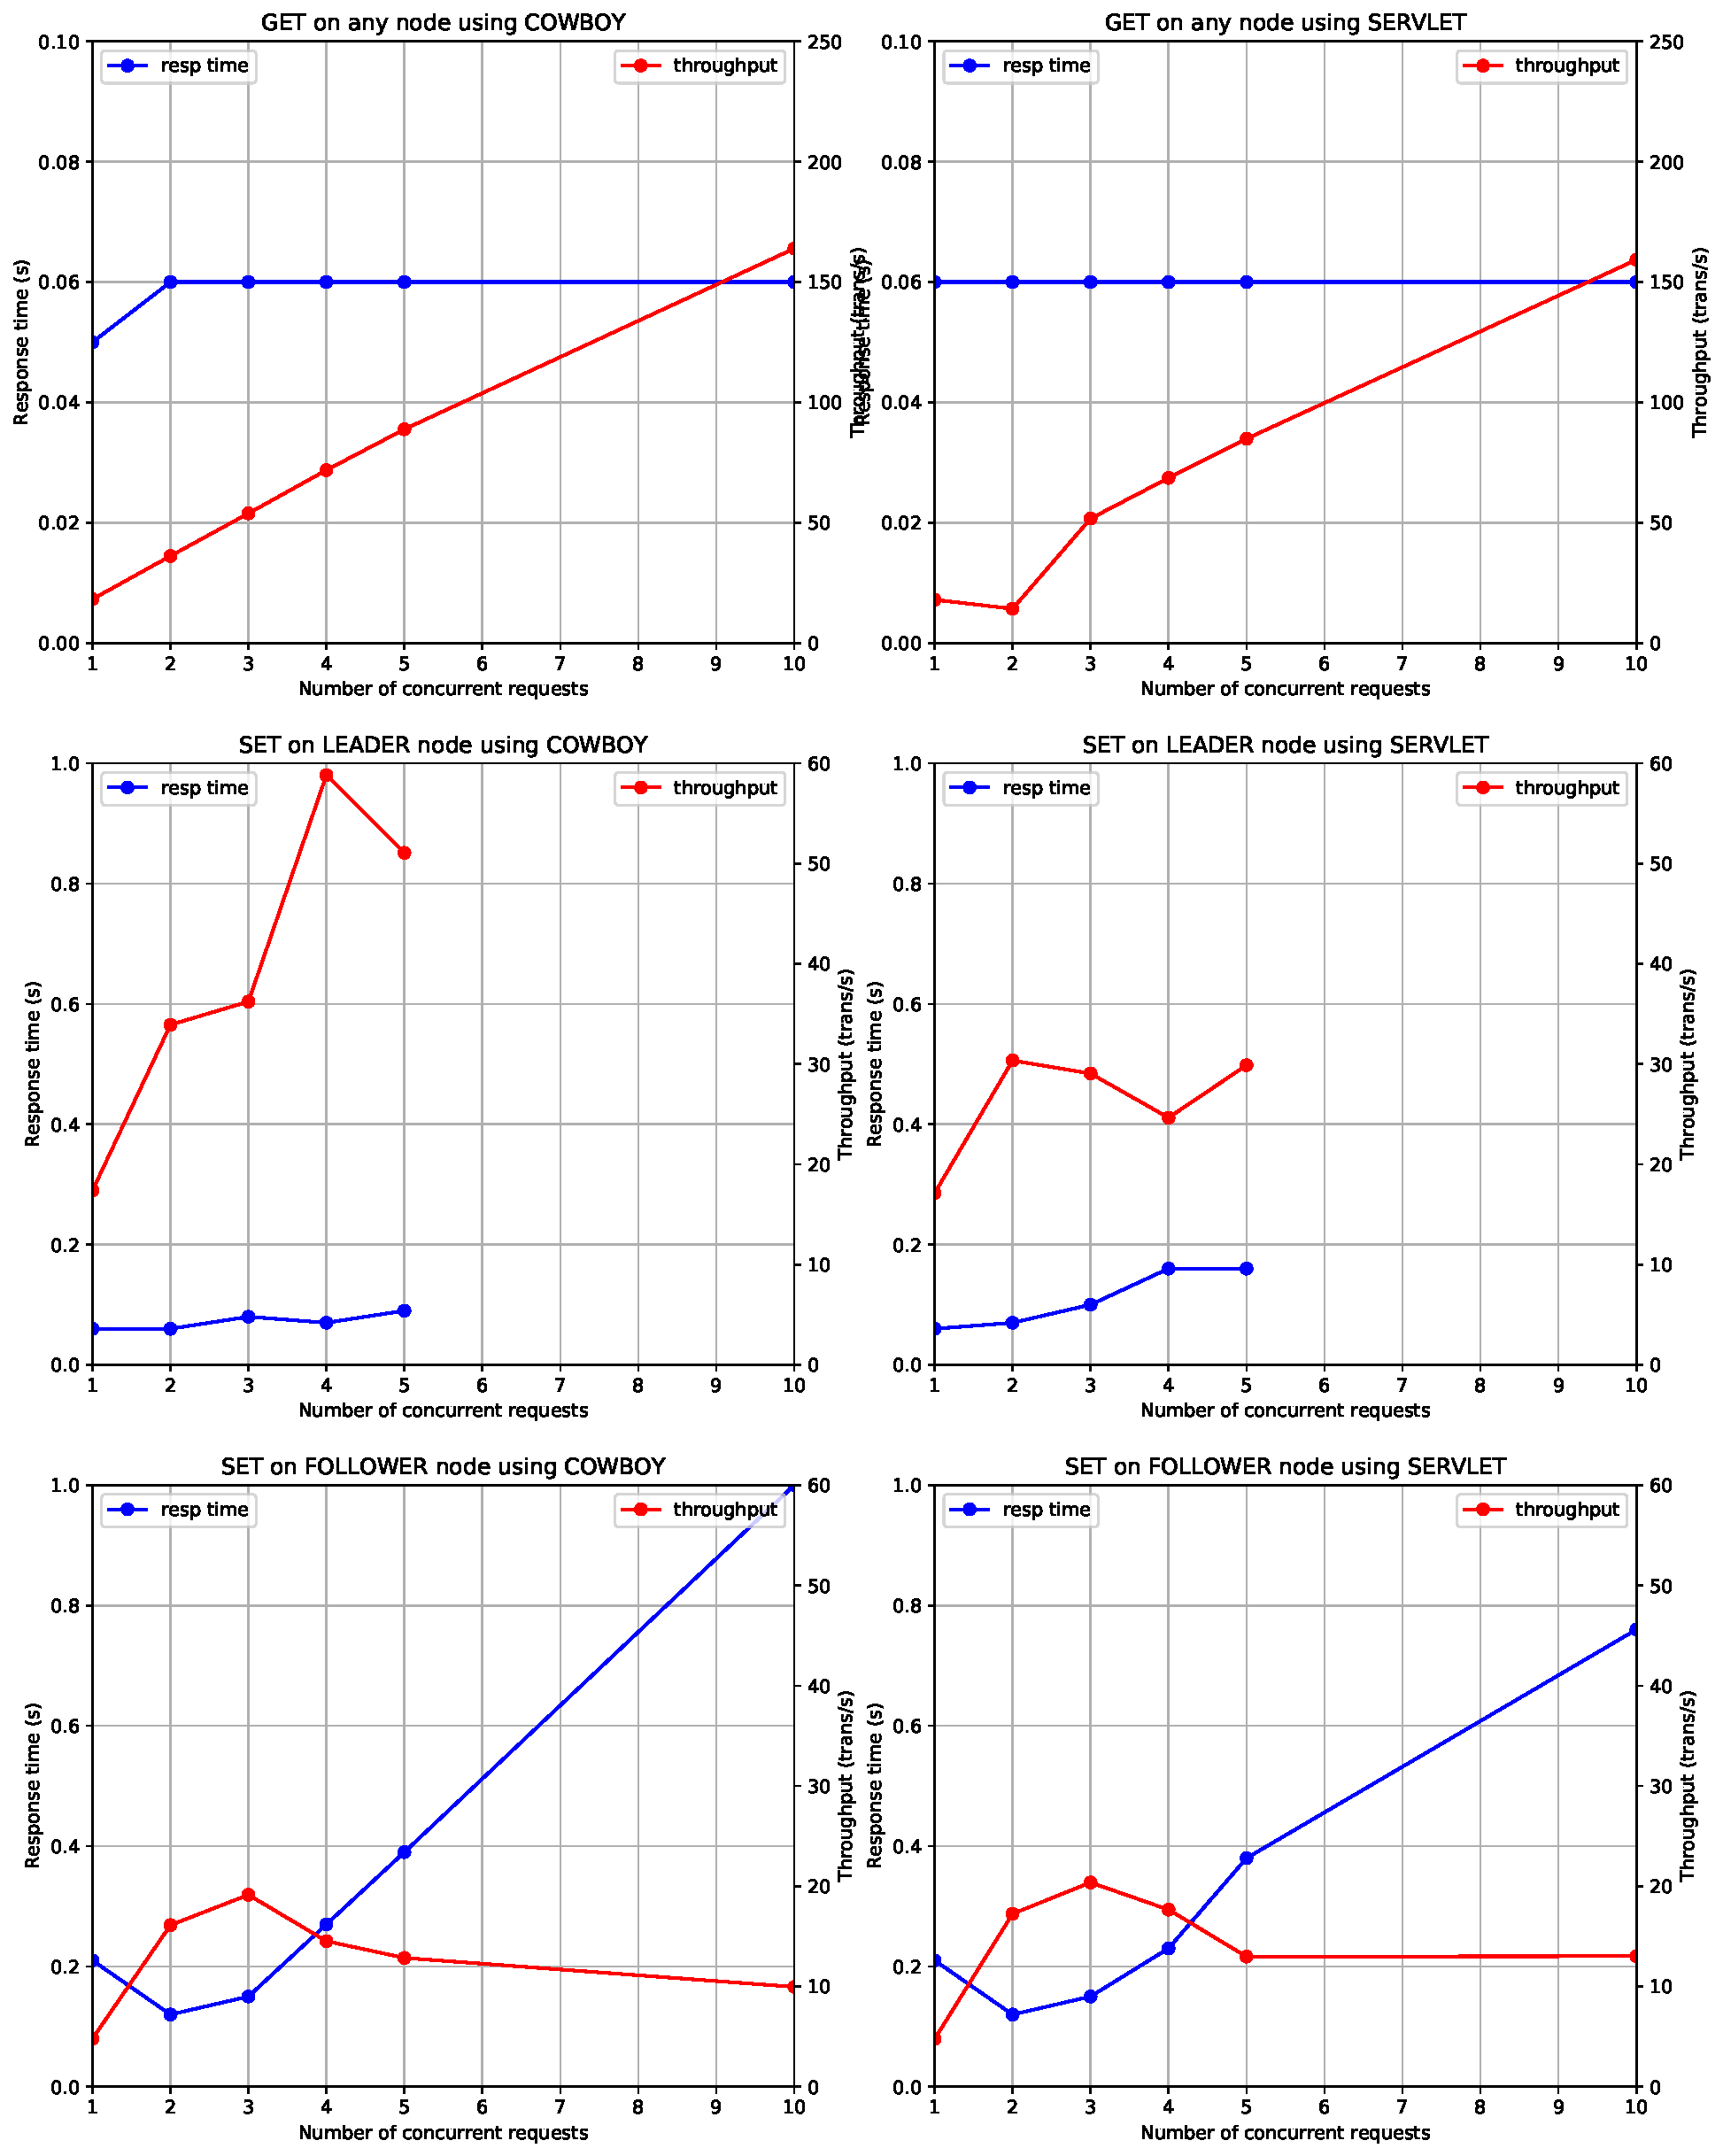
\includegraphics[width=\textwidth]{plot.pdf}
    \caption{Response time and throughput for different operations (GET or SET), on different nodes (LEADER or FOLLOWER), for both servers (COWBOY or SERVLET) by varying the number of concurrent users (requests). The SET on LEADER plots stop at 5 concurrent requests since at 10 the leader loses its leadership since its VM (single core) gets overwhelmed and it does not respond in time to FOLLOWER.}
    \label{fig:plot}
\end{figure}

Figure~\ref{fig:plot} shows the results of the experiments.  In particular we 
can note that:
\begin{itemize}
    \item GET requests are much faster that SET since the KV-Store can directly
        reply.
    \item SET requests on LEADER are much faster than on FOLLOWER. This is due 
        to the fact that the LEADER commits before any FOLLOWER does.
    \item SET requests on FOLLOWER are much faster with 2 concurrent users than 
        with only one. This is due to the fact that commits are carried with 
        the next \texttt{append\_entries} RPC.
    \item COWBOY is slightly faster than SERVLET on most cases since it is more lightweight.
    \item SERVLET is slightly faster than COWBOY on SET requests on FOLLOWER, probably due to its pooling of EJBs which can send multiple requests at a time. This effect is not evident in the other cases probably due to the slowness of committing to a follower.
\end{itemize}

Our testing confirmed the good performance on read-only workloads and its 
weakness for write-heavy ones. There is still room for improvement in its 
efficiency, though.


\subsection{Resilience test}
For this test, we wanted to assess that, in case the current leader dies, 
requests to the other nodes would be interrupted only for a small time 
interval, according to the \emph{electionTimeout}. In order to do so, we 
sent a flow of requests to a follower node and, while the requests where 
running, killed the leader. We repeated this experiment several times and 
confirmed that a new leader is promptly elected within the 
\emph{electionTimeout} (which was in the range 150ms-300ms) in our case.


\end{document}
